\documentclass[xetex]{beamer}

\mode<presentation> {
  \usetheme{Frankfurt}
  \setbeamercovered{transparent}
}

\usepackage{xunicode}
\usepackage{xltxtra}
\usepackage[czech]{babel}
\usepackage{palatino}
\usepackage{graphicx}

\usepackage{listings}
\lstset{language=bash,
        numbers=left,
        numberstyle=\tiny,
        showstringspaces=false,
        aboveskip=-40pt,
        frame=leftline
        }

\title{Kyberšikana\\Cyberbullying}

\author{Ondřej Profant}
\institute[Piráti]{Česká pirátská strana}
\date{\today}

\begin{document}

\begin{frame}
  \titlepage
\end{frame}

\begin{frame}
  \frametitle{Osnova}
  \tableofcontents
\end{frame}	

\begin{frame}
  \begin{block}{Disclaimer}
  Jsem si vědom toho, že definice, taxonomie etc. jsou nuda.

	\medskip

	Též vím, že každému z vás je jasné, že se ho problematika netýká.

	\medskip

	Proto uvítám diskusi a sám se pokusím o trochu větší nadhled a~lehkost přednášky. 

	\medskip

	Občas možná budu odbočovat, avšak rozhodně tím téma nechci zlehčovat. Pokouším se jen téma podat co nejpřístupnější formou.
	\end{block}
\end{frame}

\section{Prostředí}
\begin{frame}
	\frametitle{Prostředí}
	
	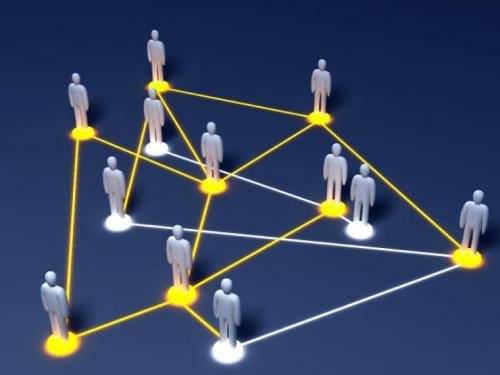
\includegraphics[scale=0.5]{soc.sites.jpg}
\end{frame}
\begin{frame}
	\frametitle{Prostředí}
	
	Sociální sítě: 
		\begin{itemize}
			\item velmi snadné (a líbivé) zpřístupnění možností Internetu (text, audio, video, informace).
			\item $\Rightarrow$ mnoho (technicky i sociálně) neznalých uživatelů
			\item komunikovat lze jak veřejně, tak skrytě (odpadá běžná soc. ochrana)
			\item ohromné počty uživatelů: 1 mld FB, 0.5~mld Twitter, 1.5~mil lide.cz
		\end{itemize}
		
	Nicméně terčem nejsou jen „komplexní“ sociální sítě. Oblíbené jsou i samostatné blogy, galerie etc.
\end{frame}

\section{Vymezení pojmu}
\begin{frame}
 \frametitle{Definice}
	\begin{block}{Kyberšikana}
	 Zneužití ICT (informačních komunikačních technologií), zejména pak mobilních telefonů a~internetu, k~takovým činnostem, které mají někoho záměrně vyvést z~rovnováhy.
	\end{block}

	\bigskip	

	Velmi tenká hranice mezi neškodným vtípkem, nepříjemným vtípkem a mezi šikanou.
\end{frame}

\subsection{Formy}

\begin{frame}
 \frametitle{Formy}
	\begin{itemize}
		\item komentáře, spam (typicky pod blogy)
		\item zveřejňování osobních dat, údajů, citlivých informací (např.~sexting)
		\item sledování (stalking)
		\item hrozby, výhružky (trolení)
		\item systematické poškozování práce/tvorby (trolení, popřípadě až útoky)
	\end{itemize} 
\end{frame}

\subsection{Rozdíly}

\begin{frame}
 \frametitle{Základní rozdíly oproti AFK šikaně}
 Kyberšikana je:
 \begin{itemize} 
		\item snažší
		\item anonymnější
		\item špatně se rozlišuje mez
		\item v rámci digitálního světa nezná hranic
		\item naopak je striktně oddělena od světa reálného
 \end{itemize}
\end{frame}

\begin{frame}
	\frametitle{Zákeřnost}
	\begin{itemize}
		\item neuvěřitelně špatně se rozlišuje počátek
		\item pokud je útočník chytrý, tak ho není lehké odhalit
		\item nikdo další o~ni nemusí vědět (nejsou zde fyzické projevy)
	\end{itemize}
\end{frame}

\begin{frame}
	\frametitle{Zajímavé rozdíly – šikana organizací}

	Kyberšikana nezasahuje jen jednotlivce.

	\bigskip

	Populární je i u organizací – komerčních, veřejných i~např. náboženských.
\end{frame}

\begin{frame}
	
\includegraphics[scale=0.6]{announce.jpg}
\end{frame}

\begin{frame}
	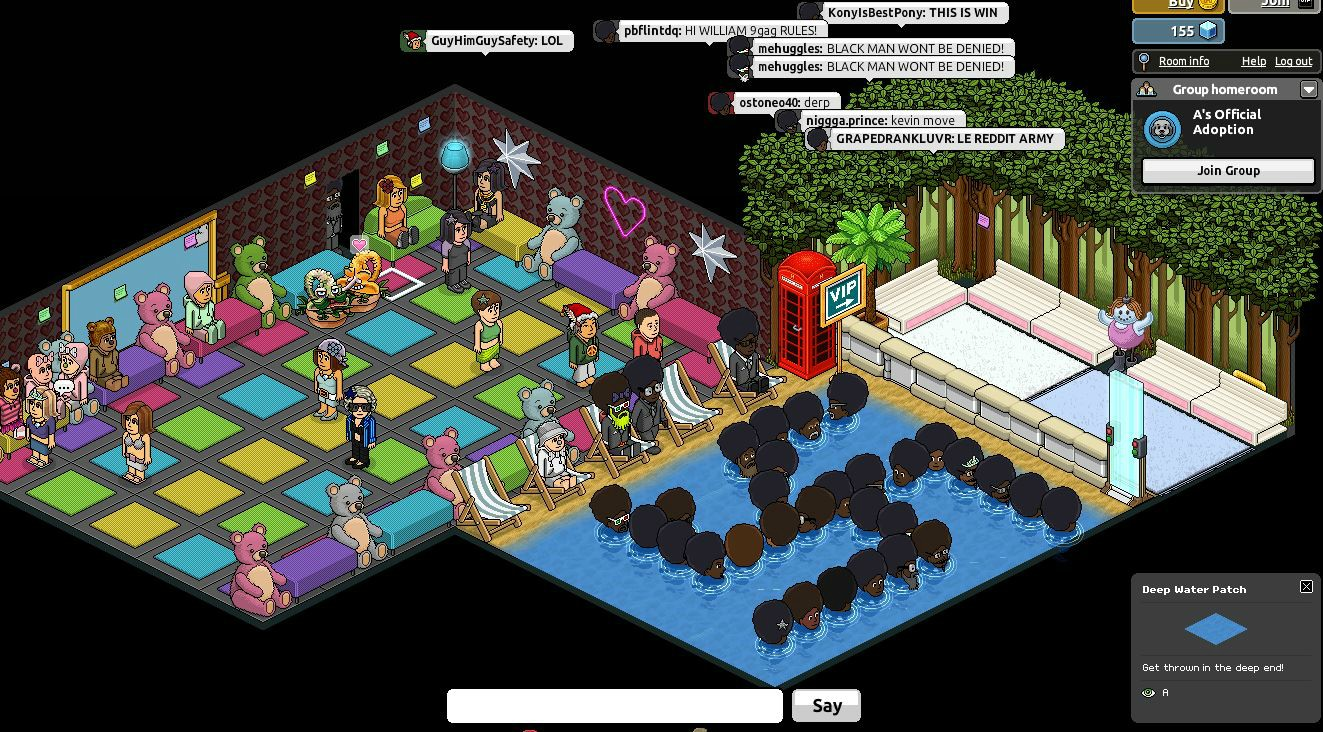
\includegraphics[scale=0.25]{habbo-hotel.jpg}
\end{frame}

\begin{frame}
	Útok na hru Habbo hotel je prvním větším a známějším případem.

	\bigskip

	Později útok na MasterCard, Visa, PayPal, Amazon (operation Payback).

	\bigskip

	Nemusí se vždy jednat jen o korporace, např. může jít i~o~církev (scientologové - operation Chanology)
\end{frame}

\section{Známé příklady kyberšikany}
\subsection{Ghyslain Raza}
\begin{frame}
  \frametitle{Ghyslain Raza}

	Rok: 2003
	
	Věk: 14 let

	Země: Kanada

	Dopady: Dlouhodobé psychiatrické lečení, mimosoudní vyrovnání

	Provedení: Šíření a remixování videa

	Základní informace: \url{http://cs.wikipedia.org/wiki/Star\_Wars\_kid}
\end{frame}

\subsection{Patrick Ryan Halligan}
\begin{frame}
	\frametitle{Patrick Ryan Halligan}
	
	Rok: 2003

	Věk: 13 let

	Země: USA

	Dopady: sebevražda

	Provedení: nejdříve fyzická šikana, později fiktivní známost přes internet

	Základní informace: \url{http://en.wikipedia.org/wiki/Suicide\_of\_Ryan\_Halligan}
\end{frame}

\subsection{Megan Taylor Meier}
\begin{frame}
	\frametitle{Megan Taylor Meier}

	Rok: 2006

	Věk: 13 let

	Země: USA

	Dopady: sebevražda, založení nadace proti kyberšikaně
	
	Provedení: fiktivní známost přes internet, útočníkem byla matka její bývalé kamarádky

	Základní informace: \url{http://en.wikipedia.org/wiki/Suicide\_of\_Megan\_Meier}
\end{frame}

\subsection{Anna Halman}
\begin{frame}
  \frametitle{Anna Halman}

  Rok: 2006

	Věk: 14 let

	Země: Polsko

	Dopady: sebevražda

	Provedení: napadení se sexuálním podtextem přímo ve třídě, výhružky zveřejněním
	
	Základní informace: \url{http://cs.wikipedia.org/wiki/Anna_Halman}
\end{frame}

\subsection{Jessica Logan}
\begin{frame}
	\frametitle{Jessica Logan}

	Rok: 2008

	Věk: 18 let

	Země: USA

	Dopady: sebevražda

	Provedení: přítel zveřejnil intimní fotografie po rozchodu
\end{frame}

\subsection{Tyler Clementi}
\begin{frame}
	\frametitle{Tyler Clementi}
	Rok: 2010

	Věk: 18 let

	Země: USA
	
	Dopady: sebevražda

	Provedení: natočení na kameru při pohlavním styku, posměch kvůli sex. orientaci
	
	Základní informace: \scriptsize{\url{http://www.novinky.cz/zahranicni/amerika/212886-student-spachal-sebevrazdu-spoluzaci-ho-nafilmovali-pri-styku-s-muzem.html}}
\end{frame}

\subsection{Rehtaeh Parsons}
\begin{frame}
	\frametitle{Rehtaeh Parsons}
	Rok: 2013
	
	Věk: 17 let
	
	Země: Kanada
	
	Dopady: Sebevražda
	
	Provedení: zneužita na večírku (bez trestu), 2 roky posměšků
	
	Základní informace: \scriptsize{\url{http://www.novinky.cz/zahranicni/amerika/310122-kybersikana-skoncila-smrti-divky-v-kanade-kvuli-tomu-zadrzeli-dva-mladiky.html}}
\end{frame}

\subsection{Rebecca Ann Sedwick}
\begin{frame}
	\frametitle{Rebecca Ann Sedwick}
	Rok: 2013
	
	Věk: 12 let
	
	Země: USA
	
	Dopady: Sebevražda
	
	Provedení: posměšky od spolužáků => změna školy, zrušení FB účtu, později se přihlásila na jinou soc. síť a útočníci si jí našli
	
	Základní informace: \scriptsize{\url{http://www.novinky.cz/zahranicni/amerika/313386-dvanactileta-divka-se-zabila-po-temer-rocni-sikane-na-internetu.html}}
\end{frame}


\section{Obrana}
\begin{frame}
	\frametitle{Prevence a obrana}

Prevence:
	\begin{itemize}
		\item znát prostředí
		\item hlídat citlivá (i potencionálně) data
		\item nedávat okázale najevo slabost (emocionální výlevy)
		\item tvrdě rozlišovat virtuální a~reálné prostředí
		\item hlídat především reálné problémy
	\end{itemize}	

Obrana:
	\begin{itemize}
		\item nevnášet zbytečné emoce (munice pro útočníka)
		\item poznat prostředí
	\end{itemize}

	Nejlepší je aktivně se bránit, čili např. poznat digitální svět.
\end{frame}

\begin{frame}
	\frametitle{Nekrmte troly}
	
\includegraphics[scale=0.45]{feed.the.troll.png}
\end{frame}


\section{Legislativa}
\begin{frame}
	\frametitle{Legislativa}

	Velmi rozdílné pojetí mezi různými státy.

	\bigskip

	Obecně platí, že tresty by měly být flexibilní závažnosti a~reálnosti opakování činu. 
	Zde je to silně umocněno tím, že útočník si často myslí, že jen neškodně vtípkuje. 
	Svůj omyl zjistí, až když je oběť v~léčebně či dokonce mrtvá.

	\bigskip

	Zločiny jsou často způsobeny nízkou sociální inteligencí útočníka i~oběti.
	Do jisté míry lze přirovnat ke zločinům z~nedbalosti 
	(obvykle tu není úmysl či uvědomnění závažnosti situace).
\end{frame}

\begin{frame}

	Děkuji za pozornost.

	\bigskip
	
	Doplňující otázky?

	\bigskip

	\bigskip

	\scriptsize
	Copyleft Ondřej Profant, 2013. Všechna práva vyhlazena. Sdílejte, upravujte a~nechte sdílet za stejných podmínek. 

	\bigskip

	Prezentace v~úplné formě\footnote{i se zdrojovými kódy} na:\\ 
	\url{https://www.github.com/kedrigern/prezentace-cs}.

	\bigskip

	Mail: ondrej.profant -at- pirati.cz 
\end{frame}

\end{document}
